\documentclass [a4paper, 11pt, twoside] {report}

\usepackage{a4}
\usepackage{titlesec}
\usepackage{amsmath}
\usepackage{amssymb}
\usepackage{graphicx}
\usepackage{listings}
\usepackage{lscape}
\usepackage{setspace}
\usepackage[left=3.3cm,top=3cm,right=3.3cm,bottom=3cm]{geometry}

\begin{document}
\begin{titlepage}
\begin{center}

\textsc{\Large Book Chapter } \\ [2cm]

{ \huge \bfseries Software Testing in the Cloud}\\[4cm]
\textsc{\large Authors:} \\[0.5cm]

\begin{minipage}{0.4\textwidth}
\begin{flushleft} \large
Faheem Ullah\\
ETH Zurich\\
\emph{faheem@inf.ethz.ch}
\end{flushleft}
\end{minipage}
\begin{minipage}{0.4\textwidth}
\begin{flushright} \large
Manuel Oriol\\
University of York\\
\emph{morio@cs.york.ac.uk}
\end{flushright}
\end{minipage}

\vfill
{\large \today}
\end{center}
\end{titlepage}
\pagebreak

The emergence of Cloud Computing offers new and exciting opportunities for software testing, promising high performance and parallelism at low cost. The need for expensive dedicated testing servers performing long testing sessions lasting for days or weeks, might soon be a thing of the past. The same testing sessions can now be distributed across the cloud and performed in parallel in a much shorter time. With the huge amount of resources available in the cloud via Infrastructure as a Service (IaaS) providers like Amazon, the upper bound on available resources is quite high and the cost is almost negligible compared to setting up a personal computational grid or buying expensive servers to perform software testing. 

Cloud Computing employs what is known as usage-based pricing for its IaaS part. Hours purchased in the Cloud can be distributed non-uniformly in time e.g. a user can utilize a 100 server hours one day and no server-hours the next and still pay only for what has been used. Another key feature of Cloud Computing is the ability to add or remove resources at a fine grain level and within a matter of minutes (a computational unit can be added or removed within a few minutes with Amazon Elastic Computer Cloud). So users can perform a distributed testing session for a large software project within a matter of hours and only pay a very small amount for the resources utilized. 

In order to satisfy the computational needs for the York Extensible Testing Infrastructure (YETI), being developed at the University of York, United Kingdom, we decided to utilize the Amazon Elastic Compute Cloud (EC2) - which is a web service that provides re-sizeable compute capacity in the cloud \footnote{http://aws.amazon.com/ec2}. A standard on-demand EC2 computer unit\footnote{1.7 GB of memory, 1 EC2 Compute Unit (1 virtual core with 1 EC2 Compute Unit), 160 GB of local instance storage, 32-bit platform} costs under 1 cent an hour. YETI is a language agnostic random testing tool. Its reference implementation tests Java programs and is able to perform over one million method calls per minute on fast library code. YETI found bugs in the \texttt{java.lang}, iText\footnote{http://itextpdf.com/} and many more programs. YETI, however, suffers from two issues:
\begin{enumerate}
\item \textbf{Performances.} On slow code, its performance can drop to as low as $10^{3}$
method calls per minute.\footnote{Observed while testing the iText library in 
September 2009} While this might seem to be a reasonable performance, experience shows 
that a plateau in the number of faults found for a given class is generally only reached after 
$10^{5}$ method calls. For large projects (100+ classes) this might mean that testing 
code on a single computer might not reach a stable point overnight. Further, YETI also has the advantage of
using multiple seeds for the pseudo-random number generator, which has been found to improve its performance compared to using only one seed over long running sessions.
\item \textbf{Security.} Secondly, the Java binding of YETI relies on the Java security model to forbid 
undesirable side-effects. This is a reasonable assumption in most cases. However,
sometimes it is undesirable because some programs need to access files, sockets, or drivers 
directly. It is also not possible to make such assumptions in cases when YETI is testing  programs written in C.
\end{enumerate}

These two issues can both be solved if YETI is distributed over the cloud: First, testing classes in parallel
allows for distribution of tasks,  the testing of 100 classes can be distributed over 100 cores, resulting in a 10minute test rather than a 1000-minute one. Similarly, testing the same class with different seeds can also be achieved in a much shorter time if distributed over different cores and run in parallel; Second, testing classes in a dedicated virtual machine, devoid of sensitive information, means that security restrictions can be relaxed.

The prototype implementation of YETI relies on the Hadoop MapReduce framework from Apache\footnote{http://hadoop.apache.org/mapreduce/}, to distribute testing sessions on remote machines and aggregate them at the end of a desired testing session.

\section{Architecture and implementation}\label{sec:architecture}

\subsection{YETI standalone application}
YETI is an automated random testing tool for Java. A testing session consists of a sequence of calls made to methods at random using arguments generated at random.  The oracle for the tests are either contracts --when available -- or runtime exceptions/failures.

When a failure is detected the logs of the testing session are minimised to 
produce test cases for reproducing the failure. Such unit tests can then be stored and 
executed later by a unit test framework.

YETI is usually launched on the command-line. A typical call to YETI is:
{\small
\begin{verbatim}
java yeti.Yeti -Java -yetiPath=. 
          -time=10mn -randomPlus
          -testModules=String:StringBuilder 
\end{verbatim}
}

The options and arguments used in the above command have the following meaning:
\begin{description}
\item{-Java} indicates that the tested program is in Java, 
\item{-yetiPath=.} indicate that classes in the current directory (and its subdirectories) will be preloaded, 
\item{-time=10mn} indicates that the testing session will last 10 minutes, 
\item{-randomPlus} indicates that the strategy random+ will be used, and 
\item{-testModules=String:StringBuilder} indicates that 
both \texttt{String} and \texttt{StringBuilder} will be tested.
\end{description}

While testing, traces of faults found are output to the terminal for inspection by the user. For example:
{\small
\begin{verbatim}
Exception 5
java.lang.NullPointerException
 at java.lang.String.replace(String.java:2207)
\end{verbatim}
}

At the end of the testing sessions, YETI outputs generated test cases reproducing 
the faults found during the testing session as well.

Note that it is possible to avoid the overhead of keeping the 
traces in the system (and calculating the minimal test cases) by specifying 
\texttt{-nologs} to throw away all logs except exception traces, or 
\texttt{-rawlogs} to output the logs to the terminal. This comes at the cost of
not being able to generate test cases for reproducing the failures that might occur during a testing session, but still provides the exception traces. In an exploratory phase of testing, this is generally the
way to use YETI.

\begin{figure}[h]
\begin{center}
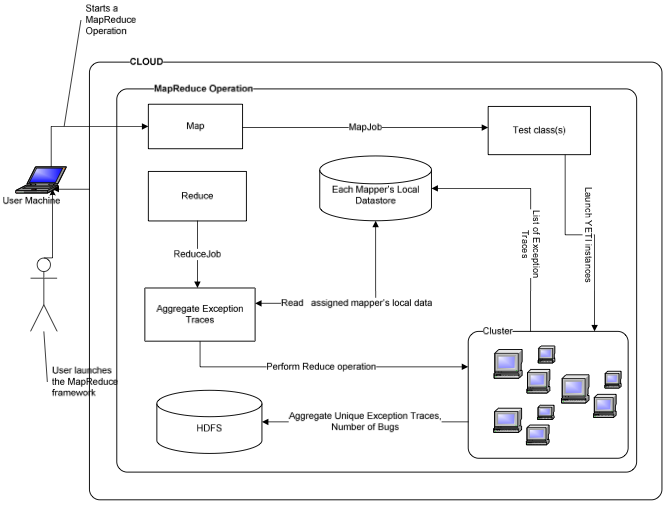
\includegraphics[width=\columnwidth]{images/YetiCloud.png}
\end{center}
\caption{YETI cloud architecture.}\label{fig:architecture}
\end{figure}


\subsection{Architecture of the cloud implementation}

As figure~\ref{fig:architecture} shows, the main architecture of YETI on the cloud 
relies on Apache's Hadoop MapRedue framework,  which is an open source implementation of Google's MapReduce framework. The framework was developed within Google for processing large amounts of raw data e.g. crawled documents or web request logs. The data is so large that it has to be distributed across thousands of machines in order to be processed within a reasonable amount of time. This distribution implies parallel computing, since the same processing is performed over all the machines with a different data set. MapReduce is a programming model and an associated implementation for processing and generating large data sets. 

Computations in the MapReduce framework take a set of input key/value pairs and produce a set of output key/value pairs. The user expresses these computations as two functions: map and reduce. The map function processes a set of key/value pairs to generate a set of intermediate key/value pairs and a reduce function which merges all intermediate values associated with the same intermediate key. The framework is designed to perform these computations in an abstract manner hiding the details of parallelism, fault-tolerance, data distribution and load balancing in a library. Figure ~\ref{fig:mapreduce}  gives and overview of the execution in Google's MapReduce framework.\footnote{ Image source: http://code.google.com/edu/parallel/img/mrfigure.png}  

\begin{figure}[h]
\begin{center}
\includegraphics[width=\columnwidth]{images/mapreduce.png}
\end{center}
\caption{Google's MapReduce framework}\label{fig:mapreduce}
\end{figure}


Hadoop MapReduce framework exactly the same. A MapReduce \emph job splits the input data into independent chunks which are then processed by the \emph map task. The output from the \emph map task serves as input for the \emph reduce task. The data required for the MapReduce job is stored on the Hadoop Distributed File System (HDFS).  

The approach employed to distribute YETI is quite simple. Testing jobs are described by calls to YETI (like the one shown before) and are stored in normal text files by the user. These will each launch YETI in standalone mode. Commands from within each file are then mapped to different machines in the cloud, launching a YETI instance and performing the desired testing session. 

After setting up the MapReduce cluster. These text files and YETI (bundled as a jar file) are uploaded to the 
HDFS on the MapReduce cluster master, which then launches individual testing machines for each text file executing the commands contained within the file in the order they appear.

At the end of the testing session, all exception traces are written back to the DFS during reduce step, which can then be downloaded to the user machine and made available to the software tester for inspection and evaluation.

Some preliminary evaluation was conducted using the Amazon Elastic Computing Cloud (EC2)\footnote{http://aws.amazon.com/ec2/}. We performed 5 jobs of 20-minutes each (a total testing time of 100 minutes) in less than 21 minutes, exhibiting comparable results with YETI's standalone execution. 
Test cases tested all the classes from \texttt{java.lang}. The number of faults found in each tested class in the distributed mode were the same as those found during standalone execution of YETI. 

By using the cloud we clearly improved the performances of YETI and reduce the testing time by 
employing more machines and distributing the jobs. 
Distributing YETI over the cloud requires uploading the files containing typical YETI calls for launching YETI in standalone mode(multiple 
YETI calls can be placed in a file resulting in the same machine testing several programs or the same program with potentially specific options/strategies for each machine), and 
YETI itself (bundled as a Jar along with the classes to be tested). Setting up a Hadoop cluster on EC2  and uploading all the required files to the 
MapReduce Master then takes under a few minutes. However, setting up the EC2 cluster for the first time might 
take some  extra time (up to 10 minutes in our tests), but subsequent testing sessions require less than a few minutes to start. 
The execution can be performed on a locally set up Hadoop cluster as well. While we did not run experiments with 
more open security models, YETI jobs were run on one-shot Ubuntu virtual machines, which solves
the potential security issues for random testing.


\end{document}
